\documentclass{aa}

\usepackage{graphicx}
%\usepackage[options]{natbib}
\usepackage{txfonts}
\usepackage{hyperref}
\usepackage{amsmath}
\usepackage{xcolor}
\usepackage{float}           % set colors

\hypersetup{ % this is just my personal choice, feel free to change things
    colorlinks,
    linkcolor={red!50!black},
    citecolor={blue!50!black},
    urlcolor={blue!80!black}}
\urlstyle{same}


\begin{document} 

   \title{The CMB power spectrum}

   \author{O. Mårem}

   \institute{Institute of Theoretical Astrophysics,  
                University of Oslo,  0315 Oslo,  Norway\\
              \email{olamaa@astro.uio.no}\\
              Github: \href{https://github.com/olamaa/AST5220}{https://github.com/olamaa/AST5220}
             }

   \date{}

   \maketitle

















































\section{Introduction}
The aim of this article is to present a simulation of the Cosmic Microwave Background (CMB) through calculations of the power spectrum (see Section \ref{section:M4}). This is a lengthy process, so it will be presented in four different milestones. The first milestone will explore the background cosmology and expansion history of the Universe, as well as examine how the uniform background densities of various matter and energy components evolve with conformal time. The goal of the second milestone will be to study the recombination history of the Universe. Our main objectives will be to calculate the optical depth and the visibility function (see Section \ref{section:M2}). These quantities are necessary for the following milestones, where we will integrate the Boltzmann-Einstein equations. We will obtain these quantities by computing the ionization fraction of hydrogen in the early universe, from which both the optical depth and visibility function can be derived. In the third milestone, we will calculate the evolution of structures in the universe from after inflation until today. In practice, this will be achieved by numerically solving the perturbed Einstein-Boltzmann equations with initial conditions from inflation. This will provide us with the time evolution of the different physical quantities of interest at different Fourier scales, denoted as $k$. A detailed derivation of the relevant equations is given in \cite{3}. Finally, with all these components in place, we will be able to compute the power spectrum of the CMB using the characterization $C_\ell$.

The report is structured into four separate sections, each with its own theory, implementation, and results section. This approach ensures that the explained concepts are not clumped together and confused with each other. The code used for the numerical simulations is written in C++ and is based on the skeleton code presented in \cite{3}. The programs have the same structure as the report with a \textbf{BackgroundCosmology}, \textbf{RecombinationHistory}, \textbf{Perturbations} and \textbf{PowerSpectum}. However, the analysis is performed in Python.


%\clearpage
\section{Milestone I}\label{section:M1}
%Some introduction about what it is all about.
In this phase, we will investigate the expansion history of a homogeneous and isotropic universe, guided by the familiar Friedmann equation (Eq. \ref{eq:Friedmann}). Our examination focuses on a universe composed of different components, including baryonic matter ($\Omega_b$), cold dark matter ($\Omega_\mathrm{CDM}$), radiation ($\Omega_\gamma$), neutrinos ($\Omega_\nu$), and dark energy ($\Omega_\Lambda$). Each component's mass/energy density is expressed relative to the critical density ($\rho_c = 3H^2/8\pi G$). Given our ultimate objective of studying the CMB, understanding the homogeneous solution of the universe is very important. The reason is that the CMB exhibits an extremely high degree of homogeneity, with perturbations of the order $10^{-5}$.

\subsection{Theory}
To compute and analyze the expansion history of the Universe, it is crucial to establish a foundation of cosmological concepts. We initiate this process by considering a flat universe (where the curvature parameter, $k = 0$). Our approach is based on the Friedmann–Lemaître–Robertson–Walker (FLRW) metric, which describes the geometry of this kind of Universe. In this metric, the line element, expressed in polar coordinates, plays an important role in our calculations. It provides a mathematical representation of the spatial relationships within the expanding universe and is given by
\begin{equation}\label{eq: ds}
    ds^2 = -c^2 dt^2 + a^2(t) \left( dr^2 + r^2(d\theta^2 + \sin^2
    \theta d\phi^2) \right),
\end{equation}
where we introduced the scale factor, denoted as $a(t)$. The scale factor represents the relative expansion of the universe over time. It serves as a crucial link between the temporal evolution of the universe and the concept of redshift. The relationship between the scale factor and redshift can be expressed as follows:
\begin{equation}\label{eq: redshift}
    1 + z = \frac{a(t_0)}{a(t)},
\end{equation}
where we have the scale factor today, denoted as $a(t_0) = 1$. To benefit computations, we introduce a parameter, namely $x$, defined as ($x \equiv \ln a$). This transformation allows us to express the scale factor in a more convenient form when dealing with phenomena that has significant variations over extended periods of time. Let us now focus on the propagation of a photon within this universe. The line element for the photon, indicating its path through spacetime, is characterized by a value of zero. Consequently, we can express Equation \eqref{eq: ds} in Cartesian coordinates using the following formulation:

\begin{equation}\label{eq: dxdt}
    \frac{dx}{dt} = \frac{c}{a(t)}.
\end{equation}
We then define the conformal time which is given by integrating
equation \eqref{eq: dxdt}
\begin{equation}\label{eq: eta}
    \eta(t) \equiv x = \int_0^{t} \frac{c dt}{a(t)}.
\end{equation}
The conformal time defines the maximum distance that particles could have traveled within the age of the Universe to reach an observer, known as the particle horizon. It provides a useful measure that relates the expansion of the Universe to a specific time. The line element can thus be expressed as a function of conformal time
\begin{equation}\label{eq: ds_eta}
    ds^2 = a^2(t) \left( -d^2\eta + dr^2 + r^2(d\theta^2 + sin^2\theta
    d\phi^2) \right).
\end{equation}
To numerically calculate the conformal time, we express it on differential form. This formulation enables us to approximate and compute the conformal time with numerical methods,
\begin{equation}\label{eq: detadt}
    \frac{d\eta}{dt} = \frac{c}{a}.
\end{equation}
The chain rule is then used for \eqref{eq: detadt} so we have
\begin{equation}\label{eq: detada}
    \frac{d \eta}{da} = \frac{c}{a^2 H} = \frac{c}{a \mathcal{H}},
\end{equation}
where the $H$ is the Hubble parameter defined as $H \equiv \frac{\Dot{a}}{a}$. Additionally, we introduce the quantity $\mathcal{H}$, defined as the product of the scale factor and the Hubble parameter, $\mathcal{H} \equiv aH$. These definitions enable us to compute the conformal time once we have knowledge of the evolution of the scale factor. We apply the chain rule once again to \eqref{eq: detada},
\begin{equation}\label{eq: detadx}
    \frac{d \eta}{dx} = \frac{c}{\mathcal{H}}.
\end{equation}
The observable linked to the expansion of the Universe is the Hubble parameter, which also can be defined using the Friedmann equations as follows:
\begin{equation}\label{eq:Friedmann}
    H = H_0 \sqrt{(\Omega_b + \Omega_m)a^{-3} + (\Omega_r +
    \Omega_\nu)a^{-4} +\Omega_\Lambda}.
\end{equation}
$H_0$ represents the present-day Hubble parameter, while $\Omega_b$, $\Omega_m$, $\Omega_r$, $\Omega_\nu$, and $\Omega_\Lambda$ denote the current relative densities of baryonic matter, dark matter, radiation, neutrinos, and dark energy, respectively. For the sake of simplicity, we will assume a neutrino density of 0 throughout all milestones. The density fractions, denoted as $\Omega_i = \rho_i /\rho_c$, represent the relative energy density of each component. These fractions are calculated by dividing the energy density of each component, denoted as $\rho_i$, by the critical density of the Universe, represented as $\rho_c$. The critical density is determined by the equation $\rho_c = 3H^2/8\pi G$, where $H$ is the Hubble parameter and $G$ is the gravitational constant. The Friedmann equations \eqref{eq:Friedmann} not only provide information about the density fractions but also describe how each component evolves over time within the expanding Universe through
\begin{align}\label{eq: dens}
    \rho_m &= \rho_{m,0} a^{-3}\\ 
    \rho_b &= \rho_{b,0} a^{-3}\\
    \rho_r &= \rho_{r,0} a^{-4}\\
    \rho_\nu &= \rho_{\nu,0} a^{-4}\\
    \rho_\Lambda &= \rho_{\Lambda,0}.
\end{align}
The cosmological parameters we will be using for all the results is the best-fit cosmology found from fits to \cite{2}.
\begin{equation}
      \boxed{
   \begin{aligned}
      h &= 0.67, \\
      T_{\rm CMB 0} &= 2.7255\,K, \\
      N_{\rm eff} &= 3.046, \\
      \Omega_{\rm b 0} &= 0.05, \\
      \Omega_{\rm CDM 0} &= 0.267,\\
      \Omega_{k 0} &= 0, \\
      \Omega_{\nu 0} &= N_{\rm eff}\cdot \frac{7}{8}\left(\frac{4}{11}\right)^{4/3}\Omega_{\gamma 0}, \\
      \Omega_{\gamma 0} &= 2\cdot \frac{\pi^2}{30} \frac{(k_bT_{\rm CMB 0})^4}{\hbar^3 c^5} \cdot \frac{8\pi G}{3H_0^2},\\
      \Omega_{\Lambda 0} &= 1 - (\Omega_{k 0}+\Omega_{b 0}+\Omega_{\rm CDM 0}+\Omega_{\gamma 0}+\Omega_{\nu 0}),
   \end{aligned}}
\end{equation}
and the density parameters evolve as 
\begin{equation}
      \boxed{
   \begin{aligned}
      \Omega_{\rm b}(a) &= \frac{\Omega_{\rm b0}}{a^3H(a)^2/H_0^2}, \\
      \Omega_{\rm CDM}(a) &= \frac{\Omega_{\rm CDM0}}{a^3H(a)^2/H_0^2},\\
      \Omega_{k}(a) &= \frac{\Omega_{\rm k0}}{a^2H(a)^2/H_0^2}, \\
      \Omega_{\nu}(a) &= \frac{\Omega_{\nu0}}{a^4H(a)^2/H_0^2}, \\
      \Omega_{\gamma}(a) &= \frac{\Omega_\gamma0}{a^4H(a)^2/H_0^2},\\
      \Omega_{\Lambda}(a) &= \frac{\Omega_{\Lambda0}}{H(a)^2/H_0^2},
   \end{aligned}}
\end{equation}
where the denotation of 0 is todays value.


\subsection{Implementation details}
For the implementation of this milestone, the main task involves completing the provided BackgroundCosmology.cpp module. Let's now examine the code structure and the completed methods and algorithms. The code begins by initializing the relevant variables, parameters, and constants required for the computations. It then proceeds to allocate arrays for various quantities of interest, including the Hubble parameter $H(x)$, the product of scale factor and Hubble parameter $\mathcal{H}(x) = aH(x)$ along with their first and second derivatives, conformal time $\eta(x)$, density parameters $\Omega_i(x)$, and distance parameters for luminosity, angular diameter, and conformal distance ($d_L$, $d_A$, $\chi$). With these initializations, we can calculate the time evolution of the different density species in the Universe using equations (\ref{eq: dens} - 14). The Hubble parameter is computed using equation \eqref{eq:Friedmann}, utilizing the provided functions H\_of\_x(x) in the \textbf{BackgroundCosmology.cpp} file, which returns $H$ for a given value of $x$. Similarly, two additional functions, Hp\_of\_x(x) and dHpdx\_of\_x(x), are used to obtain $\mathcal{H}$ and its derivative, $d\mathcal{H}/dx$, respectively. The next step involves computing the conformal time $\eta$. To achieve this, we solve equation \eqref{eq: detadx} using spline integration. However, this calculation requires an initial condition for $\eta$. We determine this initial condition by considering equation \eqref{eq: detada}. To calculate $\frac{dt}{dx}$, which provides the reciprocal of the Hubble parameter $\frac{1}{H(x)}$, we utilize the fact that we are in a radiation-dominated universe. Specifically, we have $t(x)=\frac{1}{2H(x)}$, yielding the initial condition $t_{x_\text{start}} = \frac{1}{2H(x_\text{start})}$.



\subsection{Results}
We present the results following from the implementation, beginning with a test of parameters to compare with \cite{3}.
% 1_H_dHdx
\begin{figure}[h!]
   %\hspace{-0.48cm}   
   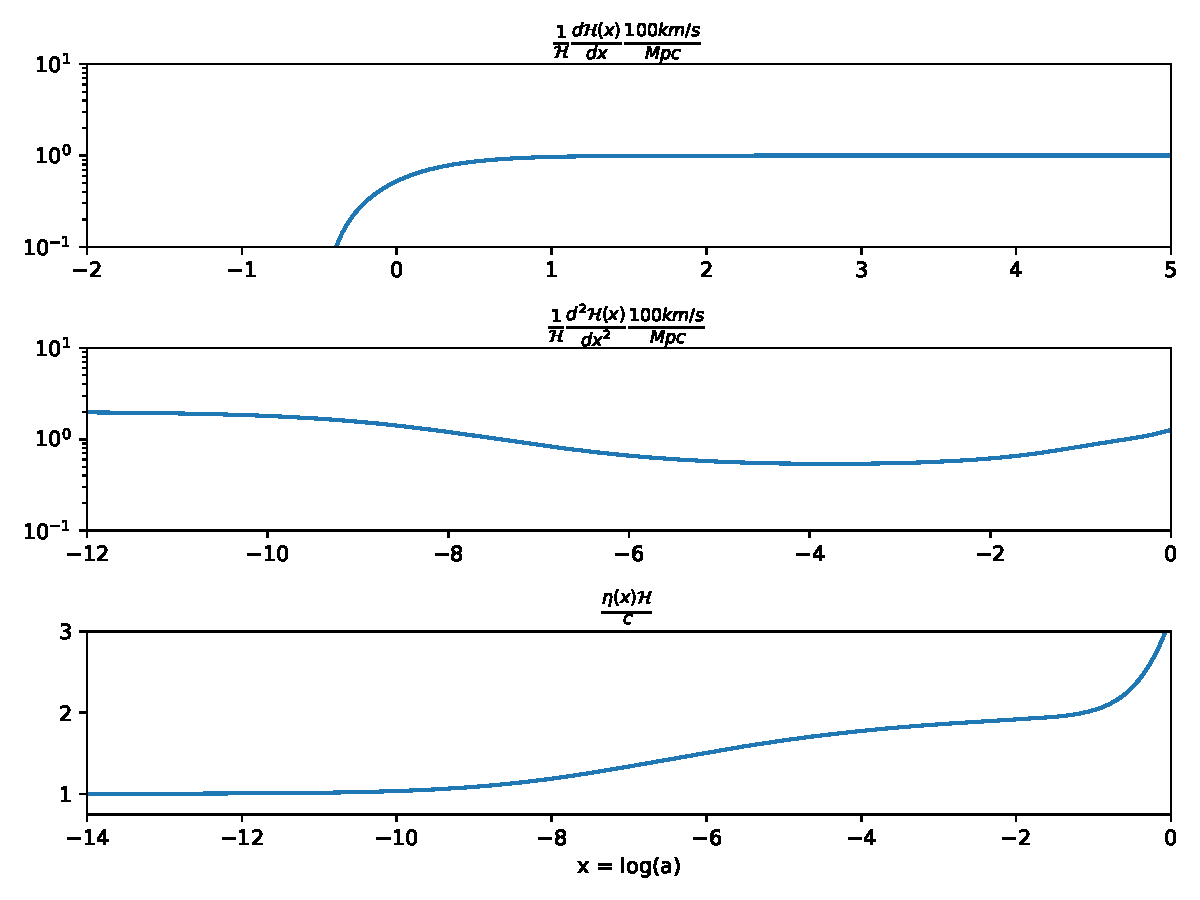
\includegraphics[scale=0.4]{Figures/milestone_1/test.pdf}
   \caption{Plots of $\mathcal{H}$ and its derivatives. We include a plot of $\frac{\eta H}{c}$ to compare our results to \cite{3}}\label{fig:M1_1_H_dHdx}
\end{figure}\\ \\ \\ \\ \\ \\ \\ \\ \\
We observe significant changes at around $x=-1$, implying a change in the Hubble parameter.

% H
\begin{figure}[h!]
   %\hspace{-0.48cm}   
   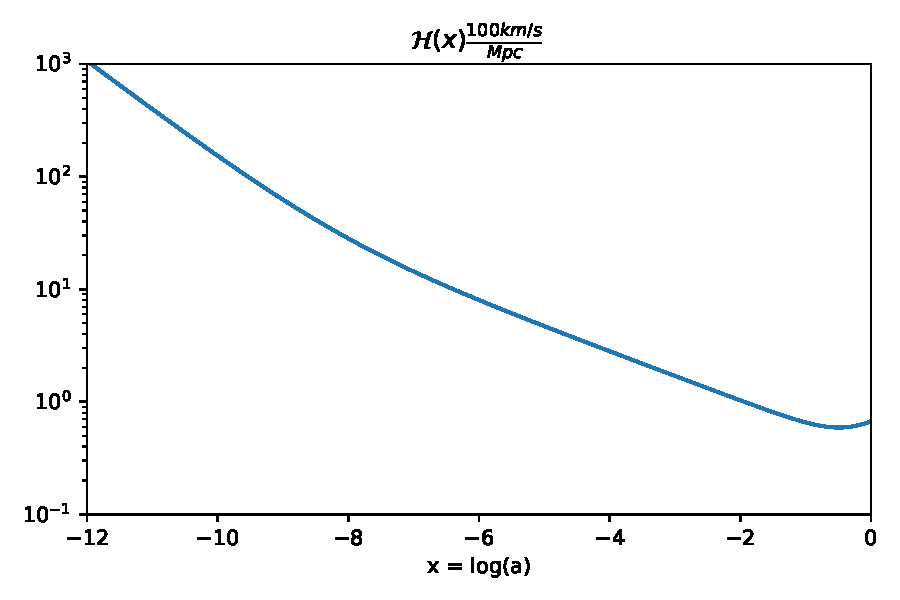
\includegraphics[scale=0.5]{Figures/milestone_1/Hx.pdf}
   \caption{The evolution of the Hubble parameter with the scale factor.}\label{fig:M1_H}
\end{figure}
The outcomes of the Hubble parameter calculation are visualized in figure \ref{fig:M1_H}. In the plot, we have represented $\mathcal{H}(x)$ as a function of $x$ using a logarithmic scale for the y-axis. This scaling choice aids in capturing the behavior of $\mathcal{H}(x)$ more effectively. The units of the plotted values are [(km/s)/Mpc], which are commonly employed when discussing the Hubble parameter. We do observe the change at $x = -1$, as the derivative of $\mathcal{H}(x)$ with respect to $x$ turns from being negative to positive  at approximately this value. 
% t
\begin{figure}[h!]
   %\hspace{-0.48cm}   
   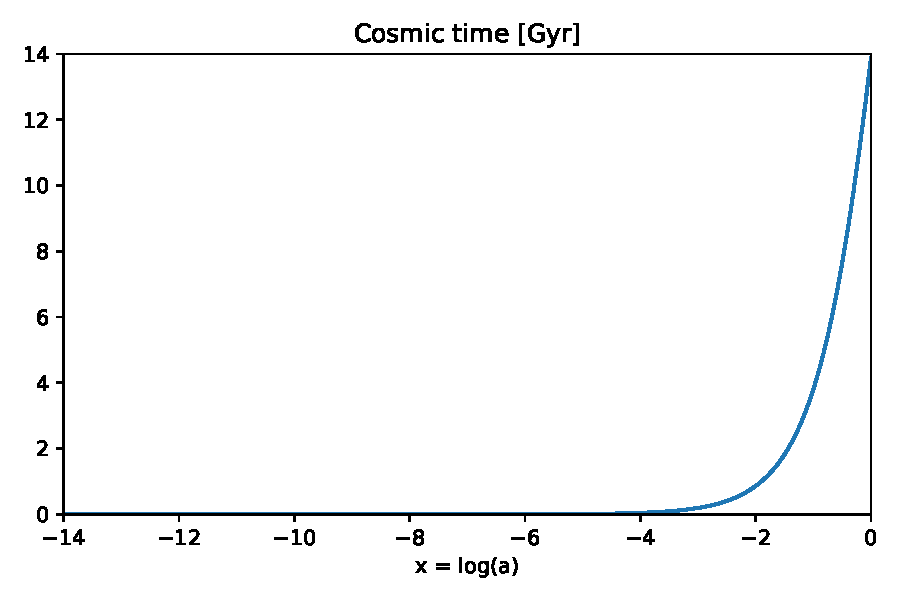
\includegraphics[scale=0.5]{Figures/milestone_1/t.pdf}
   \caption{The evolution of cosmic time with respect to the scale factor.}\label{fig:M1_t}
\end{figure}\\
In figure \ref{fig:M1_t} plot the cosmic time with respect to $x$ and observe an exponential growth as $x \rightarrow 0$. 
% eta_c
\begin{figure}[h!]
   %\hspace{-0.48cm}   
   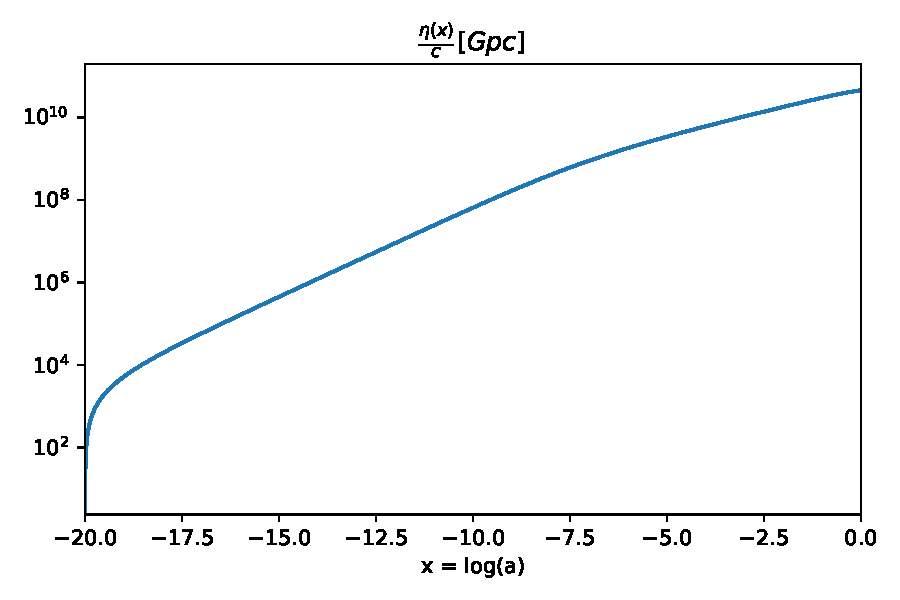
\includegraphics[scale=0.5]{Figures/milestone_1/eta_c.pdf}
   \caption{The evolution of the splined conformal time.}\label{fig:M1_eta_c}
\end{figure}\\
The calculated conformal time can be seen in figure \ref{fig:M1_eta_c}. The splined curve resolves
the entire area of $x \in [-20, 5]$. The small nudge between $x=-5$ to $x=0$ might be connected to the fact that the
Universe goes from being radiation dominated to dark matter dominated around this time, we can also draw connections to the changes in figure \ref{fig:M1_H}.

% omegas
\begin{figure}[h!]
   %\hspace{-0.48cm}   
   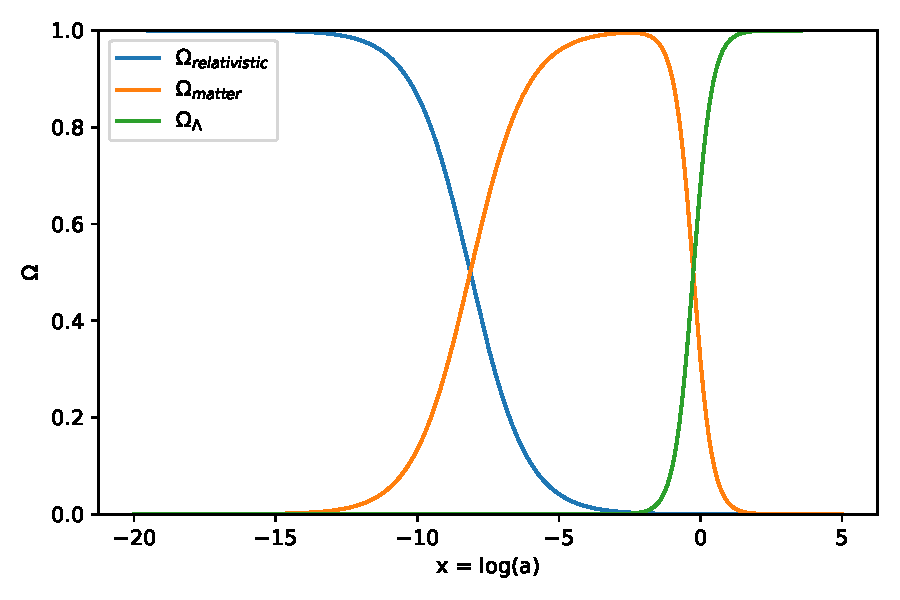
\includegraphics[scale=0.5]{Figures/milestone_1/densities.pdf}
   \caption{The evolution of the different fractional densities as a
    function of $x$.}\label{fig:M1_densities}
\end{figure}
The results of the fractional density evolution calculation are displayed in Figure \ref{fig:M1_densities}. As anticipated, the early stages of the Universe are characterized by dominance of the radiation component, $\Omega_r$, which scales with $a^{-4}$. However, around $x \approx -8$, the dark matter component, $\Omega_m$, surpasses the radiation and continues to dominate until approximately $x \approx 0$. Subsequently, the dark energy component, $\Omega_\Lambda$, becomes the dominant factor. The behavior of baryons mirrors that of dark matter, as expected, since both scale with $a^{-3}$ but with a lower overall amplitude. It is worth noting that the sum of all density components remains constant at unity throughout the evolution. Interestingly, a noteworthy observation is that the combined contribution of matter ($\Omega_m + \Omega_b$) approximately equals that of dark energy at present times.


% supernova
\begin{figure}[h!]
   %\hspace{-0.48cm}   
   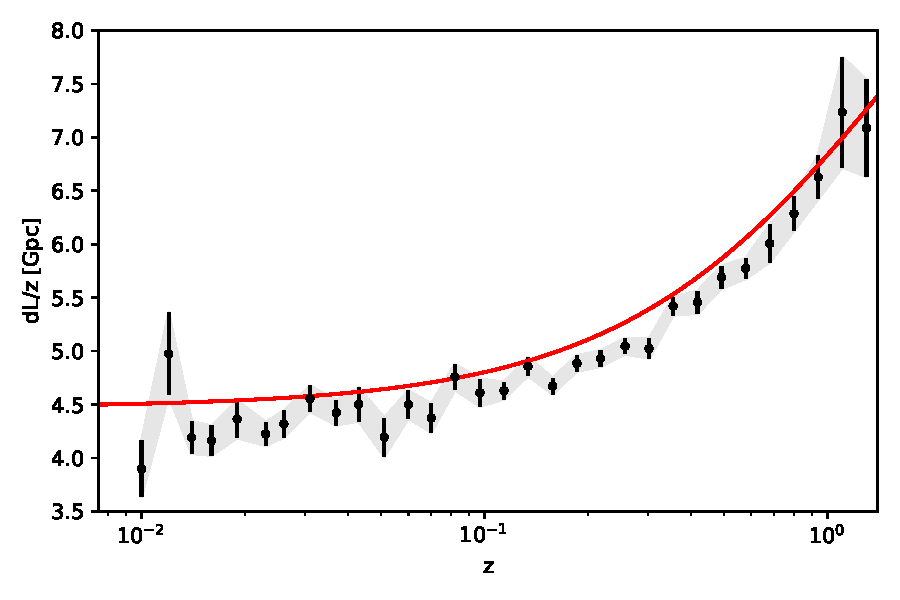
\includegraphics[scale=0.5]{Figures/milestone_1/supernova.pdf}
   \caption{Luminosity distance computed analytically compared with supernova data from \cite{1}.}
   \label{fig:M1_supernova}
\end{figure}
We have the luminosity distance in figure \ref{fig:M1_supernova}, and a comparison between the model that follows the expansion of the universe against observations from \cite{1}. We observe that even though our model is simplified to a high degree, our prediction seems reasonable.
% gaussian
\begin{figure}[h!]
   %\hspace{-0.48cm}   
   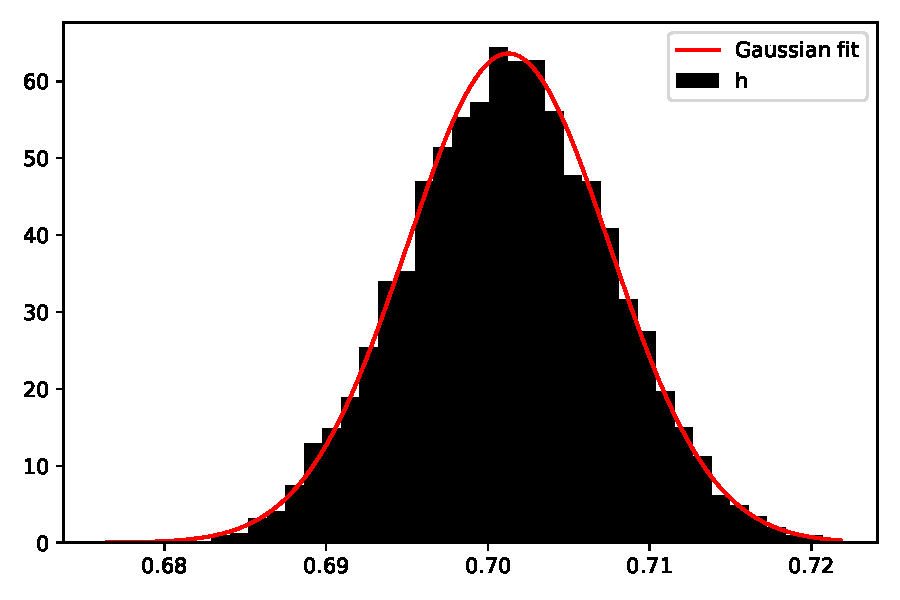
\includegraphics[scale=0.5]{Figures/milestone_1/gaussian.pdf}
   \caption{Parameter estimation of $h$ from MCMC fits to supernova data, the posterior PDF of the Hubble parameter}
   \label{fig:M1_gauss}
\end{figure}
Figure \ref{fig:M1_gauss} displays the expectation value for $h$. We observe that it does not align well with our measured value of $h=0.67$ from \cite{2}. While this indicates a poor fit, the consequences of this discrepancy are not highly significant in the context of our study.

% confidence_area
\begin{figure}[h!]
   %\hspace{-0.48cm}   
   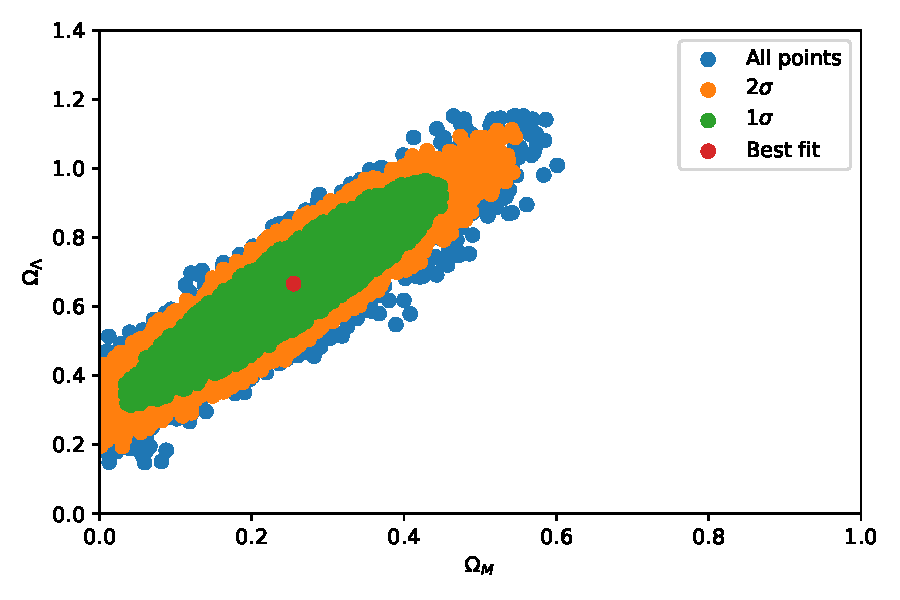
\includegraphics[scale=0.5]{Figures/milestone_1/confidence_area.pdf}
   \caption{Plots from MCMC fits to supernova data. The 1$\sigma$ and 2$\sigma$ constraints from MCMC fits to supernova data is shown in the $\Omega_M$-$\Omega_\Lambda$ plane}
\label{fig:M1_ca}
\end{figure}
The $1-2\sigma$ constraints obtained from the Markov Chain Monte Carlo (MCMC) fits provide us with reasonable results. As anticipated, we expect the present-day Universe to be dominated by dark energy, represented by $\Omega_\Lambda$, while the matter component, $\Omega_M$, is expected to be around 3. Figure \ref{fig:M1_ca} supports this expectation, showing agreement with these predicted values.
















































%\clearpage
\section{Milestone II}\label{section:M2}
In this section, our focus shifts towards investigating the properties during the recombination history of the Universe. Specifically, we will explore the transition of baryons from an ionized state to a neutral state. The primary objective of this milestone is to calculate the optical depth $\tau$ as a function of $x$, along with its derivatives. Likewise, we aim to determine the visibility function $g$ and its derivatives. These quantities will provide valuable insights into the recombination process and the state of the baryonic matter during this significant phase of the Universe's evolution.


\subsection{Theory}
In this milestone, we shift our focus to the electron number density, denoted as $n_e$. To calculate this quantity, we make use of the concept of the free electron fraction. The free electron fraction is defined as follows:
\begin{equation}\label{eq: X_e}
    X_{e} \equiv \frac{n_{e}}{n_{\mathrm{H}}}=\frac{n_{e}}{n_{b}}.
\end{equation}
Here, $n_{\mathrm{H}}$ denotes the total number density of hydrogen, which we approximate to be equal to the baryon number density, $n_{\mathrm{b}}$, by disregarding the contribution of helium. The hydrogen density can be expressed as:
\begin{equation}\label{eq: n_e}
    n_{\mathrm{H}}=n_{b} \simeq
    \frac{\rho_{b}}{m_{\mathrm{H}}}=\frac{\Omega_{b} \rho_{c}}{m_{\mathrm{H}}
    a^{3}},
\end{equation}
Here, $\rho_b$ and $\rho_c$ represent the baryon and critical densities today, respectively, while $m_\mathrm{H}$ corresponds to the mass of a hydrogen atom. Prior to recombination (at $X_e \approx 0.99$), the electron fraction can be approximated using the Saha equation:
\begin{equation}\label{eq: saha}
    \frac{X_{e}^{2}}{1-X_{e}} \simeq \frac{1}{n_{b}}\left(\frac{m_{e} T_{b}}{2
    \pi}\right)^{3 / 2} e^{-\epsilon_{0} / T_{b}}.
\end{equation}
During these early times, when the baryons and photons were tightly coupled, the baryon temperature ($T_b$) can be approximated to be equal to the photon temperature. Here, $m_e$ refers to the electron mass and $\epsilon_0$ represents the ionization energy of hydrogen.
\begin{equation}\label{eq: T_b}
    T_{b} \simeq T_{r}=\frac{T_{0}}{a}, \quad T_{0}=2.725 \mathrm{K}.
\end{equation}
As the system undergoes the process of recombination, the decoupling of photons from baryons causes a transition out of strong thermodynamic equilibrium (TE), making the Saha equation insufficient. To address this, we turn to the Peebles equation, which provides a more accurate representation of the non-equilibrium state. The Peebles equation is formulated as
\begin{equation}\label{eq: peeble}
    \frac{d X_{e}}{d
    x}=\frac{C_{r}\left(T_{b}\right)}{H}\left[\beta\left(T_{b}\right)\left(1-
    X_{e}\right)-n_{\mathrm{H}} \alpha^{(2)}\left(T_{b}\right)
    X_{e}^{2}\right].
\end{equation}
The Peebles equation incorporates essential aspects of particle physics that improve the accuracy of calculating $X_e$. Within this equation, we introduce substitutions represented by $C_r$, $\beta(T_b)$, and $\alpha^{(2)}(T_b)$, which are defined
\begin{align}\label{eq: subs}
    C_{r}\left(T_{b}\right)&=\frac{\Lambda_{2 s \rightarrow 1
    s}+\Lambda_{\alpha}}{\Lambda_{2 s \rightarrow 1
    s}+\Lambda_{\alpha}+\beta^{(2)}\left(T_{b}\right)}, \\
    \Lambda_{2 s \rightarrow 1 s}&=8.227 \mathrm{s}^{-1}, \quad
    \Lambda_{\alpha}=H \frac{\left(3 \epsilon_{0}\right)^{3}}{(8 \pi)^{2} n_{1
    s}},\\
    n_{1 s} &=\left(1-X_{e}\right) n_{H}, \\ \beta^{(2)}\left(T_{b}\right)
    &=\beta\left(T_{b}\right) e^{3 \epsilon_{0} / 4 T_{b}},\\
    \beta\left(T_{b}\right)&=\alpha^{(2)}\left(T_{b}\right)\left(\frac{m_{e}
    T_{b}}{2 \pi}\right)^{3 / 2} e^{-\epsilon_{0} / T_{b}},\\
    \alpha^{(2)}\left(T_{b}\right)&=\frac{64 \pi}{\sqrt{27 \pi}}
    \frac{\alpha^{2}}{m_{e}^{2}} \sqrt{\frac{\epsilon_{0}}{T_{b}}}
    \phi_{2}\left(T_{b}\right),\\
    \phi_{2}\left(T_{b}\right) &\simeq 0.448 \ln \left(\epsilon_{0} /
    T_{b}\right).
\end{align}
It is important to note that the equations presented above are expressed in natural units. The electron density plays a significant role as it enables us to calculate the optical depth of the Universe.
\begin{equation}\label{eq: tau}
    \tau(\eta)=\int_{\eta}^{\eta_{0}} n_{e} \sigma_{T} a d \eta^{\prime},
\end{equation}
The optical depth, denoted as $\tau(\eta)$, can be understood as the probability of a photon undergoing scattering with an electron. In the context of the equations mentioned earlier, $\sigma_T$ represents the Thompson cross section, $\eta$ corresponds to the conformal time, and the prime ($'$) denotes differentiation with respect to $x$. Additionally, we can express the optical depth in a differential form, given by:

\begin{equation}
\tau' = \frac{d\tau}{dx} = -\frac{n_e \sigma_T a}{\mathcal{H}},
\label{eq: tauprime}
\end{equation}

This differential form allows for easier numerical computation of the optical depth. Once we have obtained the optical depth, it enables us to investigate another important quantity during Milestone 2, known as the visibility function.
\begin{align}
g(\eta)&=-\dot{\tau} e^{-\tau(\eta)}=-\mathcal{H} \tau^{\prime}
e^{-\tau(x)}=g(x)\label{eq: g},\\
\tilde{g}(x) &\equiv-\tau^{\prime}
e^{-\tau}=\frac{g(x)}{\mathcal{H}(x)}.\label{eq: g_tilde}
\end{align}
Here, the scaled visibility function $\tilde{g}$ is defined, and $\dot{\tau}$ represents the derivative of the optical depth with respect to time. The visibility function is normalized such that:
\begin{equation}
    \int_{0}^{\eta_{0}} g(\eta) d \eta=\int_{-\infty}^{0} \tilde{g}(x) d x=1.
\end{equation}
This normalization implies that the visibility function $\tilde{g}$ provides the probability for an observed photon to have undergone scattering at a specific conformal time $\eta$. Throughout our calculations, we will be using $\tilde{g}$ as it allows us to work with functions of $x$. Therefore, when referring to the visibility function or $g$, we will be referring to equation \eqref{eq: g_tilde}.


\subsection{Implementation details}
The implementation for Milestone 2 consists of completing the \textbf{RecombinationHistory.cpp} module which considers quantities and calculations related to recombination.

The code for Milestone 2 has a similar structure to that of Milestone 1. It begins by initializing parameters and arrays necessary for the calculations, including arrays for electron density $n_e$, electron fraction $X_e$, and the parameter $x$.

The code assumes the initial regime to be the Saha regime, where the Universe is in strong thermodynamic equilibrium (TE). It then enters a for-loop that iterates over 4000 points between 0 and 1. In each iteration, the code checks if $X_e < 0.99$, indicating the transition out of TE. At this point, Peebles' equation \eqref{eq: peeble} is used with the end of the Saha regime as the initial condition. Peebles' equation is a first-order differential equation, and it is solved using an ODE routine similar to the one used in Milestone 1. The code includes a function to compute the right-hand side (RHS) of \eqref{eq: peeble}, which is then passed to the ODE routine to obtain the solution for $X_e$.

Once $X_e$ is obtained, the electron number density $n_e$ is computed by solving equation \eqref{eq: X_e}. To ensure efficient and accurate calculations for arbitrary values of $x$, a spline interpolation of the logarithm of $n_e$ is performed. The use of logarithmic spline is suitable because $n_e$ can vary significantly over different orders of magnitude.

With the electron density $n_e$ available, the next step is to compute the optical depth $\tau$. This is achieved by solving equation \eqref{eq: tauprime}, which is another ordinary differential equation. The solution process is similar to that of Peebles' equation, using an ODE solver routine and a subroutine to compute the right-hand side (RHS) of \eqref{eq: tauprime}.

The optical depth is defined such that $\tau = 0$ at the present time. This value is used as an initial condition, and the ODE solver routine is employed to solve \eqref{eq: tauprime} and obtain the solution for $\tau$. After obtaining $\tau$, a spline interpolation is performed to facilitate future evaluations.

Furthermore, the code implements the calculation of the first and second derivatives of the optical depth, $\tau'$ and $\tau''$, respectively. These derivatives are computed using the \textit{.deriv\_x} and \textit{.deriv\_xx }properties. These derivatives are necessary for computing the visibility function $g$ and will be useful in subsequent milestones.

In the final part of the implementation, our focus shifts to the computation of the visibility function, $g$. Unlike the electron density and optical depth, the visibility function can be directly obtained by using the values of $\tau$ and $\tau'$. This simplifies the implementation of equation \eqref{eq: g_tilde}. To compute the derivatives $g'$ and $g''$, we follow a similar approach as we did for the optical depth, utilizing the same methods.


\subsection{Results}
In Figure \ref{fig:M2_tautilde}, we observe the optical depth of the universe plotted as a function of $x = \log a$, along with its two derivatives. As expected from its definition in equation \eqref{eq: tau}, the optical depth closely tracks the behavior of the electron density. All three functions are continous and show a close alignment with each other. Notably, around $x \approx -7$ (corresponding to a redshift of $z \approx 1100$), the optical depth reaches a value of $\tau = 1$. This critical value marks the transition between an opaque and optically thick medium, indicating the point at which the universe became opaque during recombination. This finding aligns well with our understanding of the recombination process. Furthermore, the second derivative of the optical depth shows a slight increase around $x \approx -7$, likely as a consequence of recombination occurring.

\begin{figure}[h!]
   %\hspace{-0.48cm}   
   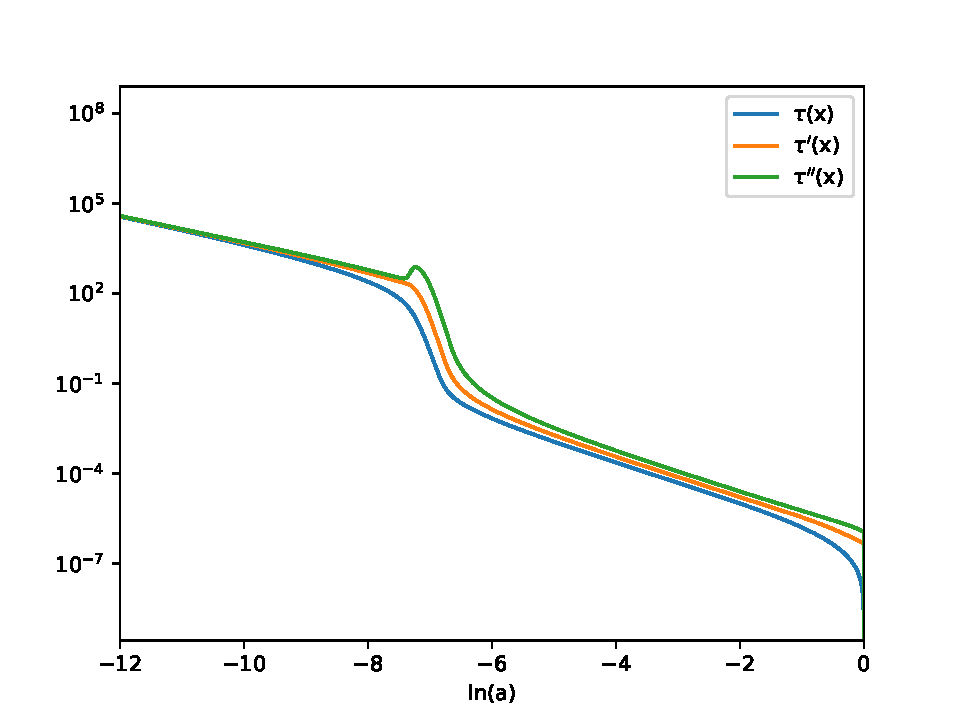
\includegraphics[scale=0.5]{Figures/milestone_2/tautilde.pdf}
   \caption{The optical depth $\tau$ along with the first and second derivatives $|\tau'|$ and $\tau''$}
    \label{fig:M2_tautilde}
\end{figure}

The cosmic ionization history is illustrated in Figure \ref{fig:M2_Xe}, which displays the fractional electron density as a function of $x$. Prior to recombination, the free electron fraction remains approximately equal to 1, indicating a fully ionized state. However, as recombination takes place, the free electron fraction experiences a rapid decline. Notably, we observe a change in the rate of this decrease around $x = -7$, marking a significant shift in the ionization dynamics.
\begin{figure}[h!]
   %\hspace{-0.48cm}   
   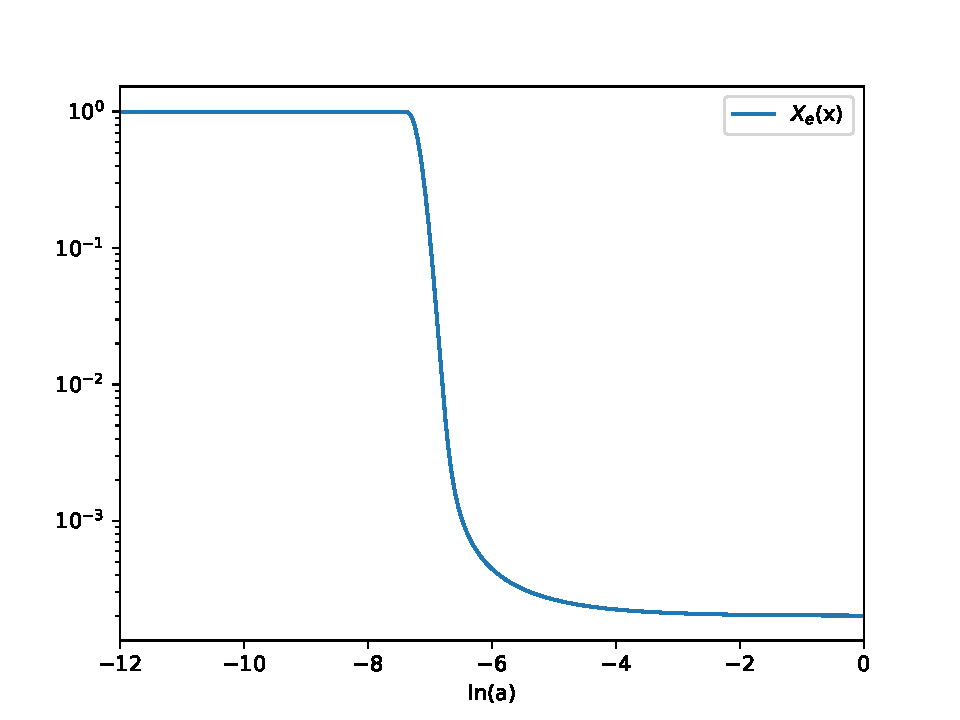
\includegraphics[scale=0.5]{Figures/milestone_2/Xe.pdf}
   \caption{The free electron fraction $X_e$ as a function of the scale factor $a$.
    The Saha equation \eqref{eq: saha} is used to obtain the values prior to
    $X_e \leq 0.99$ while the Peebles equation \eqref{eq: peeble} is
    integrated to obtain the remaining values}
    \label{fig:M2_Xe}
\end{figure}
The results of the visibility function calculations are presented in Figure \ref{fig:M2_gtilde}. Before this point, the universe was too dense for scattering to take place. At $x \approx 7$, we observe a peak in the visibility function. As explained in the theory section, the visibility function represents the probability distribution of when a cosmic microwave background (CMB) photon, observed today, underwent its last scattering event. The peak in the visibility function indicates that this scattering event predominantly occurred around a redshift of $z \approx 1100$, corresponding to the time of recombination. This peak signifies the moment when photons were effectively decoupled from the scattering process, leading to the formation of the CMB radiation that we observe.
\begin{figure}[h!]
   %\hspace{-0.48cm}   
   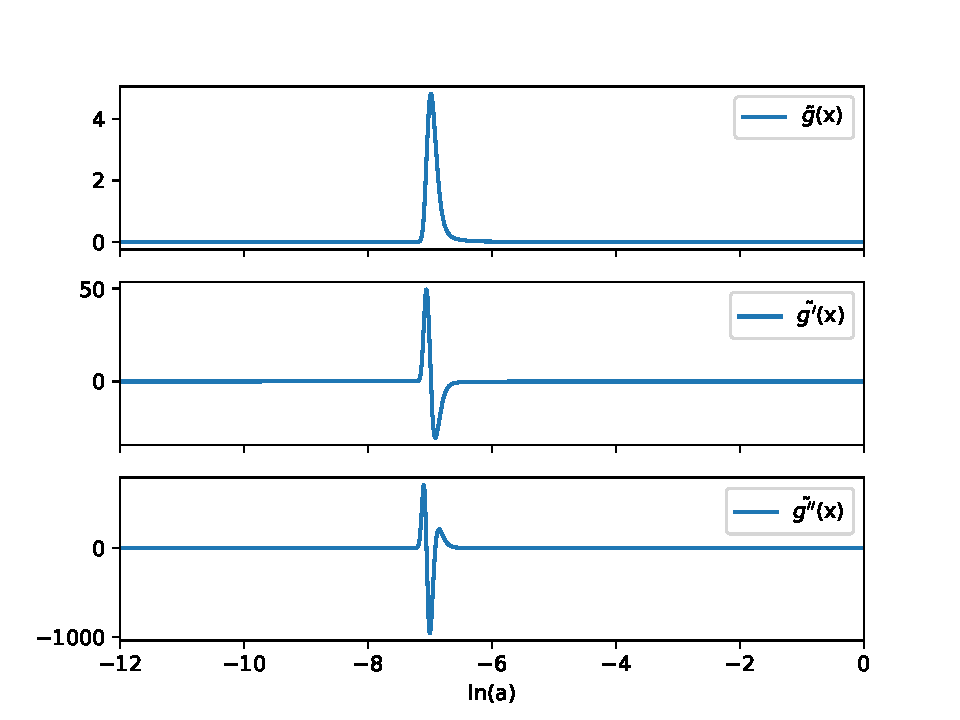
\includegraphics[scale=0.5]{Figures/milestone_2/gtilde.pdf}
   \caption{The visibility function $g$ along with the first and second
    derivatives $g'/10$ and $g''/300$. The scaling of $g'$ and $g''$ are
    chosen to make the curves fit into the same figure.}\label{fig:M2_gtilde}
\end{figure}





%3333333333333333333333333333333333333333333333333333333333333333333333333333333333333333333333333333333333333333333333333333333333333333333333333333333
%3333333333333333333333333333333333333333333333333333333333333333333333333333333333333333333333333333333333333333333333333333333333333333333333333333333
%3333333333333333333333333333333333333333333333333333333333333333333333333333333333333333333333333333333333333333333333333333333333333333333333333333333
% Husk at det ikke er snakk om overdensity
%husk a snakke om tight coupling 
%husk a snakke om at vi løser fra radiation domination, men initial betingelsene er fra inflasjon p.g.a. horizon frys...
%sound hoizon vs. particle horizon

















































%\clearpage
\section{Milestone III}\label{section:M3}
The aim of this section is to calculate the photon temperature fluctuations in the universe. This is crucial for understanding the cosmic microwave background (CMB) and reconstructing its power spectrum. The CMB is a measurement of the temperature field of photons that we observe today. By studying the fluctuations in this temperature field across different times and Fourier scales, we can gain valuable insights into the underlying physics of the early universe.

The photon temperature fluctuations represent spatial variations in the density and temperature of the primordial plasma. These fluctuations arise from a variety of physical processes, such as acoustic oscillations, gravitational effects, and the growth of structure in the universe. By accurately calculating these fluctuations, we can reconstruct the CMB power spectrum, which provides information about the distribution of temperature fluctuations at different angular scales.


\subsection{Theory}
%The theory behind this milestone.
%Boltzmann equations, spherical harmonics, perturbation theory...
During the inflationary epoch in the early universe, certain regions experienced faster expansion than others due to quantum fluctuations in the inflaton field \cite{3}. These fluctuations led to variations in the energy density, which in turn introduced perturbations in the FLRW metric. By analyzing the Newtonian gauge, we can determine the initial conditions for the metric perturbations, denoted as $\Psi$ and $\Phi$. This information allows us to derive the initial conditions for the energy density perturbations of interest. \cite{3} provides further details on this matter.\\
\noindent
\\
The perturbations observed in the photon temperature field, represented by $\delta T$, and the matter field on large scales are significantly smaller compared to the background temperature $\overline{T}$. This characteristic allows us to use linear perturbation theory on the distribution functions, with the expectation that the obtained results will hold today. The perturbed distribution functions, denoted as $f_i$, for baryons, photons, and cold dark matter (CDM), can be expressed in the following form:
\[f_i(t,\vec{x},\vec{p})= \overline{f_i}(t,\vec{p}) + \delta f_i(t,\vec{x},\vec{p}),\] 
The perturbed distribution functions, denoted as $\delta f_i$, represent the deviations from the background distribution function $\overline{f_i}$. These perturbations have an impact on the energy-momentum tensor in the Einstein equations, consequently affecting the metric. As a result, the motion of particles in space and time is altered within this perturbed framework, as described in \cite{3}. Thus, we encounter a system of coupled differential equations.

To solve the perturbed Einstein-Boltzmann equations, we transform into Fourier space and use the logarithmic scale factor $x = \ln a$ as the time variable. The perturbations in the photon temperature, represented by the relative perturbation $\Theta = \delta T/\overline{T}$, are expanded into Legendre multipoles. This allows us to express the photon distribution in terms of these multipole moments, denoted as $\Theta_\ell$. Similarly, we solve for the perturbations in the CDM and baryon overdensities, defined as $\delta_\mathrm{CDM} = \frac{\delta \rho_{CDM}}{\overline{\rho}{CDM}}$ and $\delta\mathrm{b} = \frac{\delta \rho_{b}}{\overline{\rho}_{b}}$ respectively. The velocities, similar to the density perturbations, are also expressed in a dimensionless form. We follow a similar approach for their definition. However, it's important to note that in our calculations, we do not solve the equations for polarization perturbations. Additionally, we do not include perturbations associated with neutrinos in this analysis. 
\\
The initial conditions are:
$$
\boxed{
\begin{aligned}
\Psi &= -\frac{2}{3} \\
\Phi &= -\Psi \\
\delta_{\rm CDM} &= \delta_b = -\frac{3}{2} \Psi \\
v_{\rm CDM} &= v_b = -\frac{ck}{2\mathcal{H}} \Psi \\
&\text{Photons:}\\
\Theta_0 &= -\frac{1}{2} \Psi \\
\Theta_1 &= +\frac{ck}{6\mathcal{H}}\Psi \\
\Theta_2 &= -\frac{20ck}{45\mathcal{H}\tau^\prime} \Theta_1 \\
\Theta_\ell &= -\frac{\ell}{2\ell+1} \frac{ck}{\mathcal{H}\tau^\prime} \Theta_{\ell-1},\\
\end{aligned}
}
$$

with the photon equations:
$$
\boxed{
\begin{aligned}
\Theta^\prime_0 &= -\frac{ck}{\mathcal{H}} \Theta_1 - \Phi^\prime, \\
\Theta^\prime_1 &=  \frac{ck}{3\mathcal{H}} \Theta_0 - \frac{2ck}{3\mathcal{H}}\Theta_2 +
\frac{ck}{3\mathcal{H}}\Psi + \tau^\prime\left[\Theta_1 + \frac{1}{3}v_b\right], \\
\Theta^\prime_\ell &= \frac{\ell ck}{(2\ell+1)\mathcal{H}}\Theta_{\ell-1} - \frac{(\ell+1)ck}{(2\ell+1)\mathcal{H}}
\Theta_{\ell+1} + \tau^\prime\left[\Theta_\ell - \frac{1}{10}\Theta_2
\delta_{\ell,2}\right],\\ 
& \mathrm{where} \ \ 2 \leq \ell \textless \ell_{\textrm{max}} \\
\Theta_{\ell}^\prime &= \frac{ck}{\mathcal{H}}
\Theta_{\ell-1}-c\frac{\ell+1}{\mathcal{H}\eta(x)}\Theta_\ell+\tau^\prime\Theta_\ell,
\quad\quad \ell = \ell_{\textrm{max}},\\
\end{aligned}
}
$$

and the equations for cold dark matter and baryons:
$$
\boxed{
\begin{aligned}
\delta_{\rm CDM}^\prime &= \frac{ck}{\mathcal{H}} v_{\rm CDM} - 3\Phi^\prime \\
v_{\rm CDM}^\prime &= -v_{\rm CDM} -\frac{ck}{\mathcal{H}} \Psi \\
\delta_b^\prime &= \frac{ck}{\mathcal{H}}v_b -3\Phi^\prime \\
v_b^\prime &= -v_b - \frac{ck}{\mathcal{H}}\Psi + \tau^\prime R(3\Theta_1 + v_b) \\
\end{aligned}
}
$$
with metric perturbations:
$$
\boxed{
\begin{aligned}
\Phi^\prime &= \Psi - \frac{c^2k^2}{3\mathcal{H}^2} \Phi\\
&+ \frac{H_0^2}{2\mathcal{H}^2}
\left[\Omega_{\rm CDM 0} a^{-1} \delta_{\rm CDM} + \Omega_{b 0} a^{-1} \delta_b + 4\Omega_{\gamma 0}
a^{-2}\Theta_0\right] \\
\Psi &= -\Phi - \frac{12H_0^2}{c^2k^2a^2}\left[\Omega_{\gamma 0}\Theta_2\right], \\
\end{aligned}
}
$$
where $R = \frac{4\Omega_{\gamma 0}}{3\Omega_{b 0} a}$. In the early stages of the universe, there is a numerical instability issue that arises due to the multiplication of a large value of $\tau^\prime$ with a small value of $(3\Theta_1+v_b)$. This occurs during the tight coupling regime when the universe was opaque. The onset of the tight coupling regime can be determined by the simultaneous satisfaction of the following conditions: $|\tau^\prime| > 10$, $|\tau^\prime| > 10 \cdot \frac{ck}{\mathcal{H}}$, and $x \leq -8.3$. In order to address this instability, we present the modified equations below.

$$
\boxed{
\begin{aligned}
q &= \frac{-[(1-R)\tau^\prime + (1+R)\tau^{\prime\prime}](3\Theta_1+v_b)}{(1+R)\tau^\prime + \frac{\mathcal{H}^\prime}{\mathcal{H}} -1}\\
  &\frac{-\frac{ck}{\mathcal{H}}\Psi + (1-\frac{\mathcal{H}^\prime}{\mathcal{H}})\frac{ck}{\mathcal{H}}(-\Theta_0 +
2\Theta_2) - \frac{ck}{\mathcal{H}}\Theta_0^\prime}{(1+R)\tau^\prime + \frac{\mathcal{H}^\prime}{\mathcal{H}} -1}\\
v_b^\prime &= \frac{1}{1+R} \left[-v_b - \frac{ck}{\mathcal{H}}\Psi + R(q +
\frac{ck}{\mathcal{H}}(-\Theta_0 + 2\Theta_2) - \frac{ck}{\mathcal{H}}\Psi)\right]\\
\Theta^\prime_1 &= \frac{1}{3} (q - v_b^\prime).
\end{aligned}
}
$$
In the tight coupling regime, the photon multipoles with $2 \leq l$ can be expressed using the same equations as the initial conditions. However, these multipoles are very small during this regime, and for simplicity and numerical stability, we can approximate them as zero. The multipole $\Theta_2$ is calculated separately to ensure numerical stability.\\

\subsection{Implementation details}
The code follows a structured approach. It starts by defining an array for log $k$, which allows for numerical calculations over different orders of magnitudes of $k$. The initial conditions for the tight coupling regime are then set. A function is implemented to compute the RHS for $\Theta_1'$, which represents the derivative of the $\Theta_1$ multipole. This RHS function is then used in the ODE solver routine to obtain the solution for $\Theta_1'$. Next, the integration is performed from the end of the tight coupling regime to the present time. To ensure a smooth transition between the two regimes, the last value in the first regime is removed when merging the solutions. This removal of the overlap between the solutions helps in avoiding redundancy and maintaining consistency during the integration process.


\subsection{Results}

In a static universe, the formation of baryonic structures is generally not expected before recombination, as the Jeans mass depends linearly on the sound speed, which was approximately equal to the speed of light ($c$) during that time. However, immediately after recombination, the sound speed "freezes out," and the formation of structures becomes easier. In our results, we can observe that the baryon overdensity starts to continuously increase around the time of recombination ($x=-7$). This observation supports the discussion regarding the behavior of the sound speed. On the other hand, for CDM, we do not observe any oscillatory behavior at early times because CDM is pressureless, and gravity only needs to work against the cosmic acceleration. It is important to note that in some cases, the overdensity values may be less than -1, which is physically impossible by definition. However, this is not a concern in our analysis because the quantities have not been scaled to represent physical values.\\ \\
%Velocity is negative right after perturbation has rebound
%Show and discuss the results.
\begin{figure}[h!]
   %\hspace{-0.48cm}  
   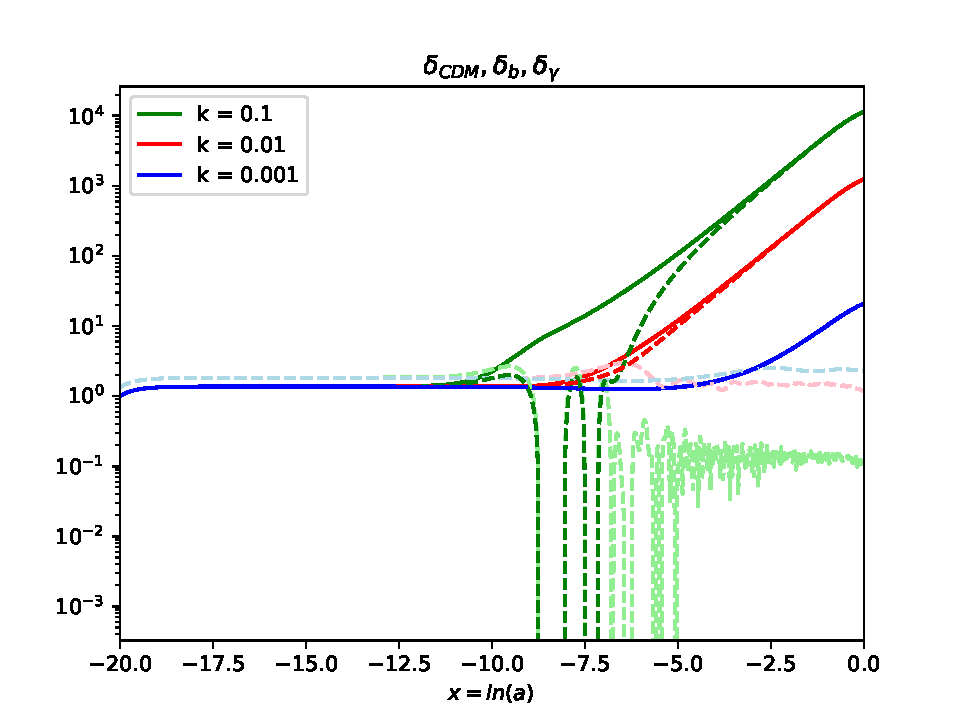
\includegraphics[scale=0.5]{Figures/milestone_3/deltas.pdf}
   \caption{The CDM overdensity, the absolute value of the baryon overdensity and the comparable photon overdensity $\delta_\gamma = 4\Theta_0$. The solid lines are for CDM and the dotted lines are for baryons while the lighter dotted lines are for the photons at three different scales, $k$. }
   \label{fig:M3_deltas}
\end{figure}

Figure \ref{fig:M3_deltas} illustrates an important concept: the reach of gravity in the universe is determined by the conformal time, denoted as $\eta$. The conformal time represents the maximum distance over which gravity can exert its influence at any given time. If the scale of interest, represented by the value of $k$, is larger than the conformal time, there won't be any correlation because the scale is causally disconnected. By considering the relationship that Fourier modes enter the particle horizon when $k\eta=1$, we can determine when a specific scale enters the particle horizon. In this case, we find that the scale $k=0.1/\mathrm{Mpc}$ enters the particle horizon at $x\sim -10$, indicating that structures on this scale become observable. In our results, we observe that the behavior of CDM aligns with this theory. Comparatively, at $x\sim -16$, CDM begins to cluster, implying that if we look at larger values of $k$, we should approach this value. The oscillations in the overdensity arise due to the interplay between gravity and pressure. Initially, gravity compresses the mass, causing it to become denser. However, as the density increases, the pressure also increases, leading to a rebound effect where the mass expands. This cycle repeats until the mass reaches the critical value known as the Jeans mass, which represents the minimum mass required for structure formation.

\begin{figure}[h!]
   %\hspace{-0.48cm}   
   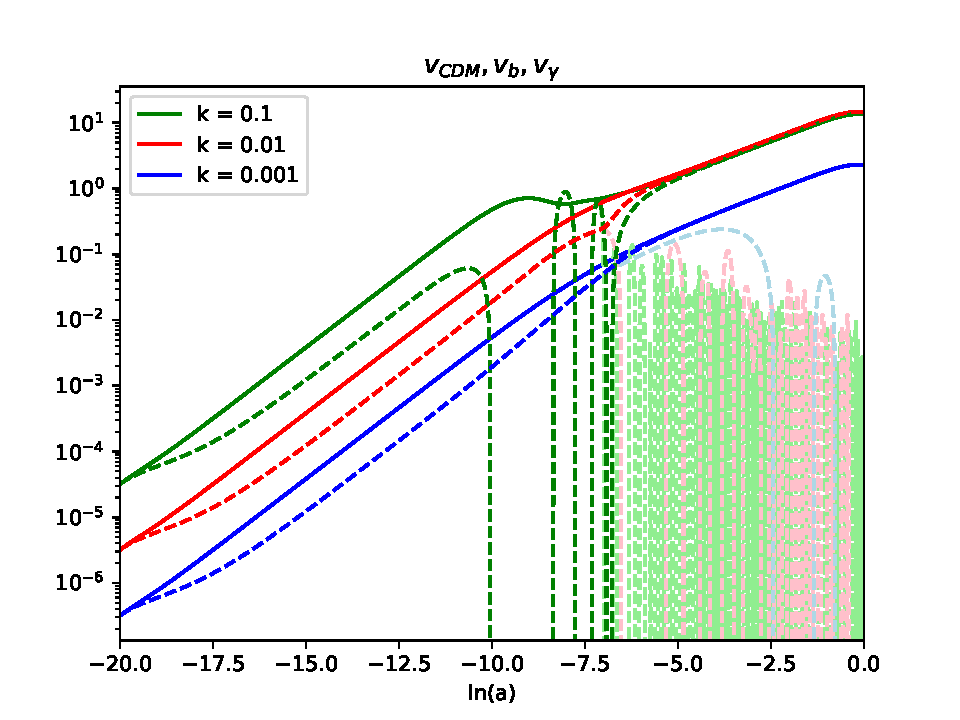
\includegraphics[scale=0.5]{Figures/milestone_3/Vs.pdf}
   \caption{The CDM velocities in solid lines, the absolute value of the baryon velocities
   in dotted lines and the photon velocity perturbation, $v_\gamma=-3\Theta_1$, at three different scales, $k$}
   \label{fig:M3_Vs}
\end{figure}
Figure \ref{fig:M3_Vs} provides insights into the behavior of the baryonic overdensity and its corresponding fluid velocity. We observe that the oscillations in the baryonic overdensity, as the mass contracts and rebounds, are accompanied by corresponding oscillations in the baryonic fluid velocity. The behavior differs based on the scale being considered. At a smaller scale, represented by the green curve, the mode enters the particle horizon earlier, resulting in a higher frequency of oscillations in the baryonic overdensity. As we move to larger scales, indicated by the red and blue curves, the modes enter the particle horizon after recombination. Consequently, the baryonic overdensity exhibits no oscillations on these larger scales. This behavior can be understood in the context of causal connectivity. When the scale is smaller than the particle horizon during recombination, there is sufficient time for oscillatory behavior to emerge. However, for larger scales that enter the horizon later, there is insufficient time for such oscillations to develop.

\begin{figure}[h!]
   %\hspace{-0.48cm}   
   \includegraphics[scale=0.5]{Figures/milestone_3/theta_2.pdf}
   \caption{The photon temperature quadrupole, $\Theta_2$, at three different scales.}
   \label{fig:M3_theta2}
\end{figure}

\begin{figure}[h!]
   %\hspace{-0.48cm}   
   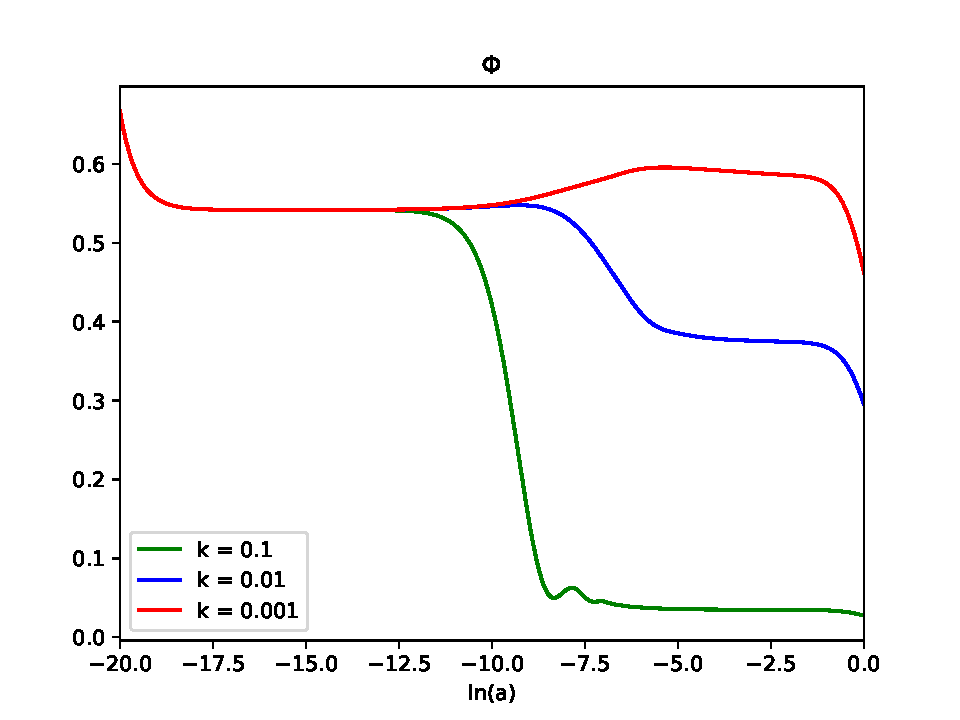
\includegraphics[scale=0.5]{Figures/milestone_3/phi.pdf}
   \caption{The gravitational potential at three different scales, $k$.}\label{fig:M3_phi}
\end{figure}

\begin{figure}[h!]
   %\hspace{-0.48cm}   
   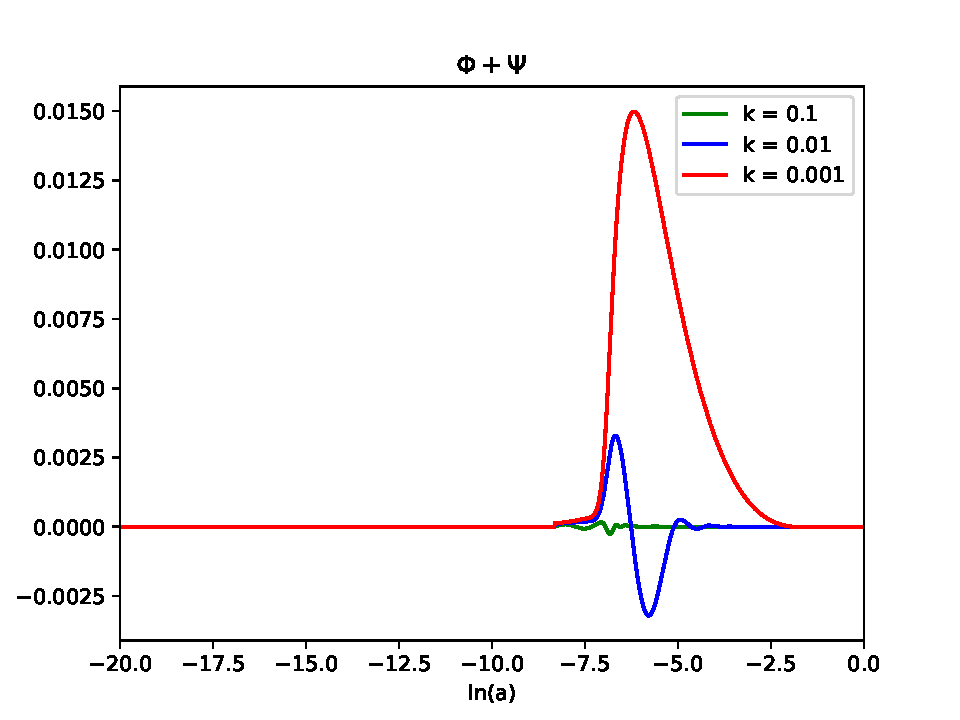
\includegraphics[scale=0.5]{Figures/milestone_3/phipsi.pdf}
   \caption{The sum of the two gravitational potentials, $\Phi$ and $\Psi$, at three different scales, $k$.}\label{fig:M3_phipsi}
\end{figure}
















































%\clearpage
\section{Milestone IV}\label{section:M4}

Up until now, we have made substantial advancements in understanding the expansion dynamics of the universe as well as determining the number density of free electrons and their influence on the mean free path of photons. Using these results, we calculated the evolution of initial perturbations since the inflationary epoch until today. With these insights, we are prepared to achieve our primary objective: namely, the derivation of the power spectrum of the Cosmic Microwave Background (CMB). Our final outcome will manifest as the power spectrum denoted by $C_\ell$, which comprehensively characterizes the power distribution across distinct angular scales within the CMB. It is noteworthy that smaller values of $\ell$ correspond to the inclusion of larger scales, whereas larger values of $\ell$ correspond to smaller scales.

\subsection{Theory}
The CMB power spectrum is defined by performing a spherical harmonics transform on the temperature field. This transform allows us to decompose the temperature fluctuations across the sky into different angular modes. Mathematically, the transform is represented as follows:
\begin{equation}
T(\hat{n}) = \sum_{\ell m}a_{\ell m}Y_{\ell m}(\hat{n}),
\end{equation}
where $\hat{n}$ is the observed direction,  $a_{\ell m}$ are the spherical harmonics coefficients and $Y_{\ell m}$ are the spherical harmonics themselves. The $\ell$ and $m$ correspond to an angular scale which determines the wavelength of a mode and the shape of the mode respectively. The CMB power spectrum is defined as
\begin{equation}
C_{\ell m} = \langle|a_{\ell m}|^2\rangle = \langle a_{\ell m}a^{*}_{\ell m}\rangle
\end{equation}
Where we assume isotropy, and thus be able to reduce the number of indices to $\ell$ because of rotational invariance. To obtain $T(\hat{n})$, we need to Fourier transform the temperature field $\theta_l(k, x)$ today, which we calculated in Section \ref{section:M3}. We already have resolved the temperature field up to $\ell = 6$, but we are interested in much more precise scales, up to $\ell_{\text{max}}=2000$ preferably. Calculating this would be tedious, and take a long time if it were not for \cite{4}, where a technique called line-of-sight integration (LOS) was presented. The proposal was to begin with integrating $\dot{\Theta}$, and then expand in multipoles instead of first expanding the full temperature field in multipoles and then solve the coupled equations. For more information of this procedure, see \cite{4}\&\cite{5}. The final expression becomes 
\begin{equation}
\Theta_\ell(k, x=0) = \int_{-\infty}^{0}\tilde{S}(k, x)j_\ell\left[k(\eta_0 - \eta)\right]dx.
\end{equation}
The integral is known as the transfer function where $\tilde{S}(k, x)$ is the source function. It is defined by
\begin{equation}
\begin{aligned}
\tilde{S}(k, x) &= \tilde{g}\left[\Theta_0 + \Psi + \frac{1}{4}\Pi\right] + e^{-\tau}\left[\Psi' - \Phi'\right] \\
&- \frac{1}{k}\frac{d}{dx}\left(\mathcal{H}\tilde{g}v_b\right) + \frac{3}{4k^2}\frac{d}{dx}\left[\mathcal{H}\frac{d}{dx}\left(\mathcal{H}\tilde{g}\Pi\right)\right],
\end{aligned}
\end{equation}
where the first term is the Sachs-Wolfe contribution which describes the temperature fluctuations at the last scattering surface defined by $\tilde{g}$. The $\Psi$ corresponds to the photons losing energy due to the gravitational field. We will set the $\Pi$ term equal to the temperature dipole $\Theta_2$ as it is correction due to polarization through $\Pi = \Theta_2 + \Theta^P_0 + \Theta^P_2$. The second term is the integrated Sachs-Wolfe contribution. This term includes time-varying potentials. The third term is the Doppler term which covers the interaction between photons and baryonic matter, and the final term is a polarization correction term. The $j_\ell(x)$ term are the spherical Bessel functions which are responsible of projecting the 3D temperature field characterized by $k$ onto a 2D sphere characterized by $\ell$.\\

In order to get to the actual CMB power spectrum from the transfer function we need to do two things. Firstly, we need to square $\Theta_\ell(k)$ (since $C_\ell$ is the square of the Fourier coefficients). After that we need to multiply with $P(k)$ which is the primordial power spectrum from inflation. This is a fix to our previous normalization where we normalized the Einstein-Boltzmann equations with the initial condition $\Phi = 1$. We then end up with the following expression for the power spectrum
\begin{equation}\label{eq: C_l P}
    C_{\ell}=\int \frac{d^{3} k}{(2 \pi)^{3}} P(k) \Theta_{\ell}^{2}(k).
\end{equation}
Most inflationary models predict a primordial power spectrum on the form
\begin{equation}
\frac{k^{3}}{2 \pi^{2}} P(k)=\left(\frac{c k}{H_{0}}\right)^{n-1},
\end{equation}
where $n$ is the spectral index of scalar perturbation. Solving this for $P(k)$ and inserting into equation \eqref{eq: C_l P}, we get the final CMB power spectrum expression 
\begin{equation}
    C_{\ell}=\int_{0}^{\infty}\left(\frac{c k}{H_{0}}\right)^{n-1} \Theta_{\ell}^{2}(k) \frac{d k}{k}.
\end{equation}


\subsection{implementation}
We have implemented a class that takes in BackgroundCosmology, RecombinationHistory and a Perturbations object to compute the temperature field today. We had to add the source function to section \ref{section:M3}, to be able to do the LOS integration. The method we chose was the trapezoidal rule. For this approximation to be good, we need a lot of evaluation points, we therefore use $10^9$. To make this process more efficient, we chose different regions for the integration. These regions will be limited by the scales we look at, and will have different number of points, not linked to the integration. After the LOS integration is completed, we have all the ingredients we need to calculate the power spectrum, $C_\ell$ by $C_\ell$.


\subsection{Results and discussion}
In order to check if the source function has been correctly implemented, we attempt to recreate figure 3 in \cite{5} where he has plotted the integrand of the transfer function for $\ell = 100$ and $k = 340H_0$. The results are seen in figure \ref{fig:M4_source}.


\begin{figure}[h!]
   %\hspace{-0.48cm}   
   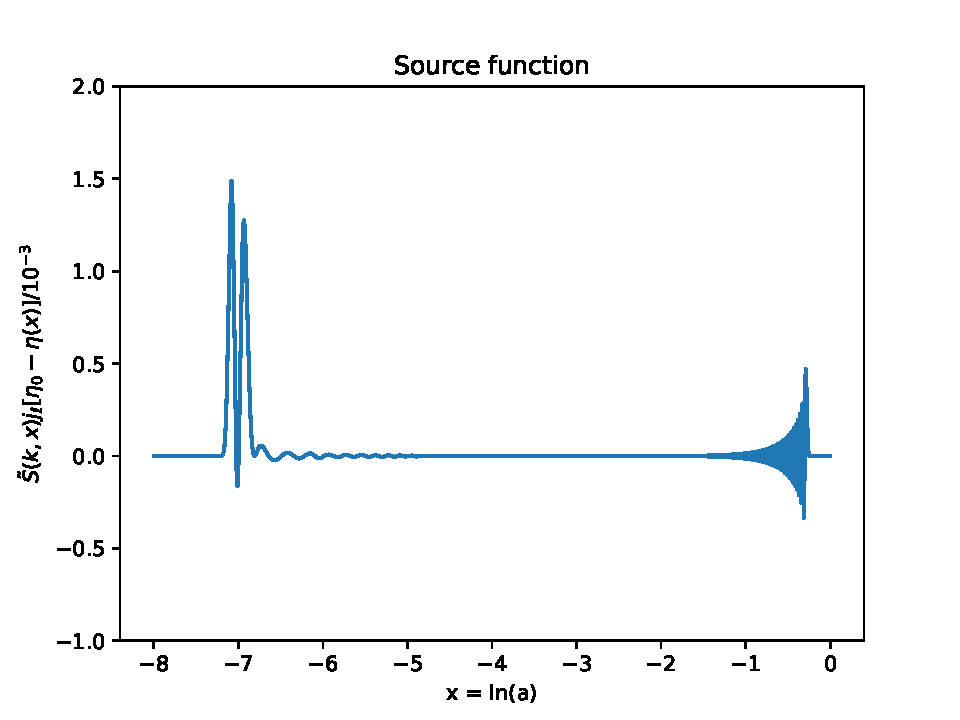
\includegraphics[scale=0.5]{Figures/milestone_4/source_function.pdf}
   \caption{The source function multiplied with the Bessel function}
   \label{fig:M4_source}
\end{figure}
We observe a similar behaviour to the source function in \cite{5}. 
\\
We proceed by plotting the transfer function for 5 different values of $\ell$. The results of this is seen in figure \ref{fig:M4_ustf}.
\begin{figure}[h!]
   %\hspace{-0.48cm}   
   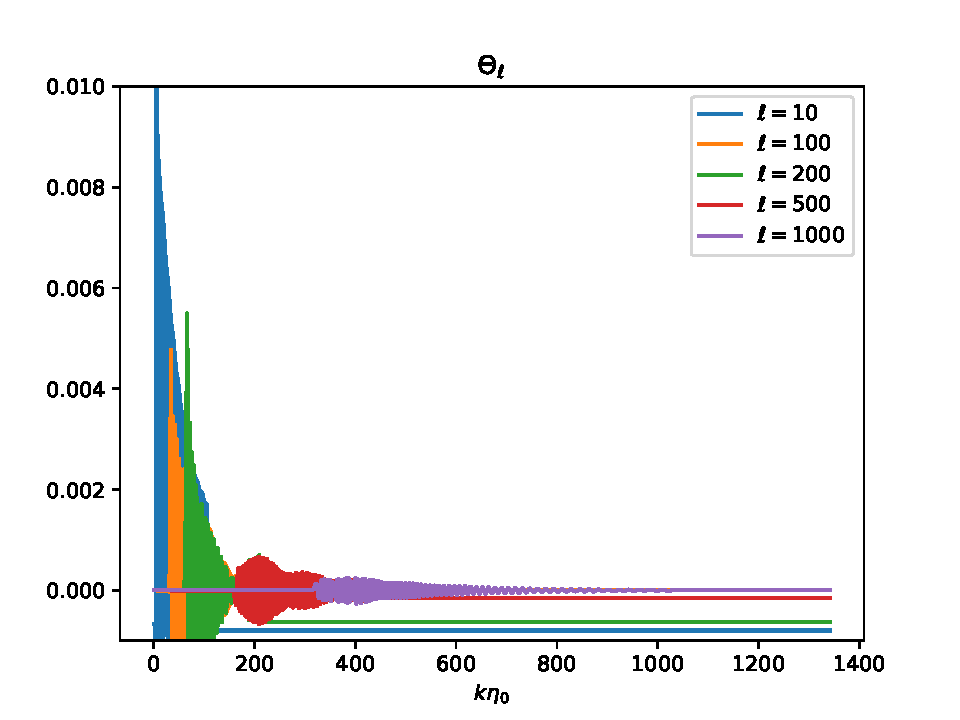
\includegraphics[scale=0.5]{Figures/milestone_4/unscaled_transfer_function.pdf}
   \caption{The transfer function plotted as a function of $k$ for 5 different values of $\ell$.}
   \label{fig:M4_ustf}
\end{figure} \\
We observe that different values of $\ell$ for the transfer function correspond to different scales in Fourier space. For small values of $\ell$ we see that large scales dominate the transfer function, and correspondingly for high $\ell$'s, small scales provide the significant contribution. It also appears as the the spread of the transfer function increases as a function of $\ell$. The $\ell = 10$ scale has a much higher amplitude than the other $\ell$'s which is a bit worrying. This might suggest that something breaks down for low $\ell$'s in our code.

In order to better be able to study how the actual contribution of the transfer function to the $C_\ell$'s, we will plot the spectrum integrand $\Theta_\ell (k)^2/k$. The results of this is seen in figure \ref{fig:M4_stf}
\begin{figure}[h!]
   %\hspace{-0.48cm}   
   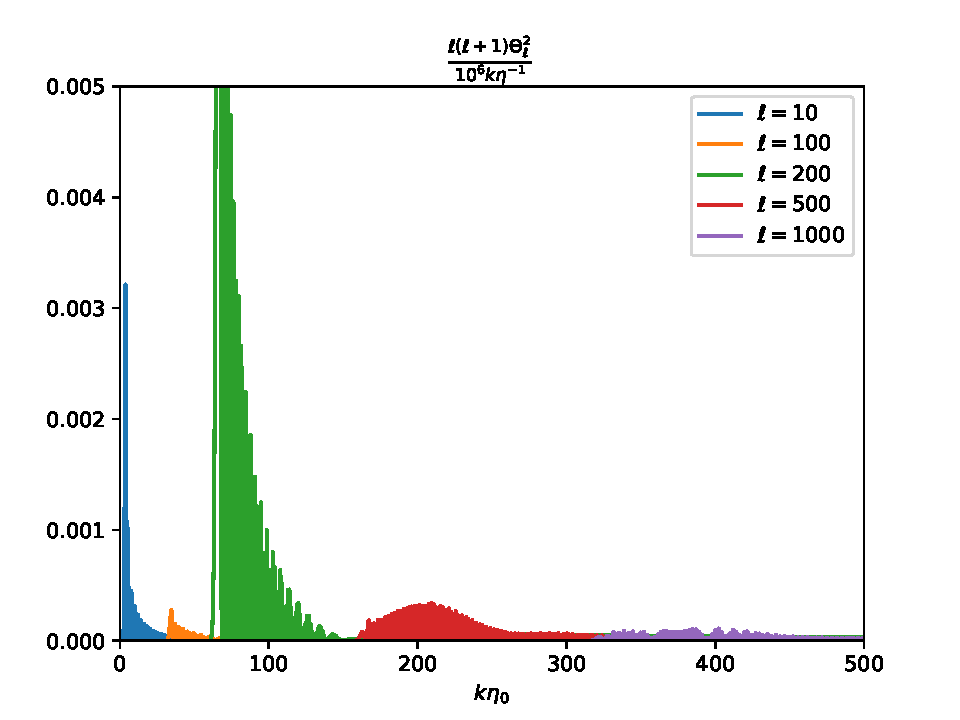
\includegraphics[scale=0.5]{Figures/milestone_4/scaled_transfer_function.pdf}
   \caption{The spectrum integrand plotted as a function of $k$ for 5 different values of $\ell$. The integrand is multiplied with $\ell(\ell +1)$ to increase the amplitude of the large $\ell$'s.
   }\label{fig:M4_stf}
\end{figure}
This plot is better at indicating which specific values of $k$ the different $\ell$ integrands contributes to. Out of the $5$ different scales, we see that the largest contribution occurs around $\ell \approx 200$. Now that we have studied the functions from which the CMB power spectrum is constructed, we are ready to plot the spectrum. 





\begin{figure}[h!]
   %\hspace{-0.48cm}   
   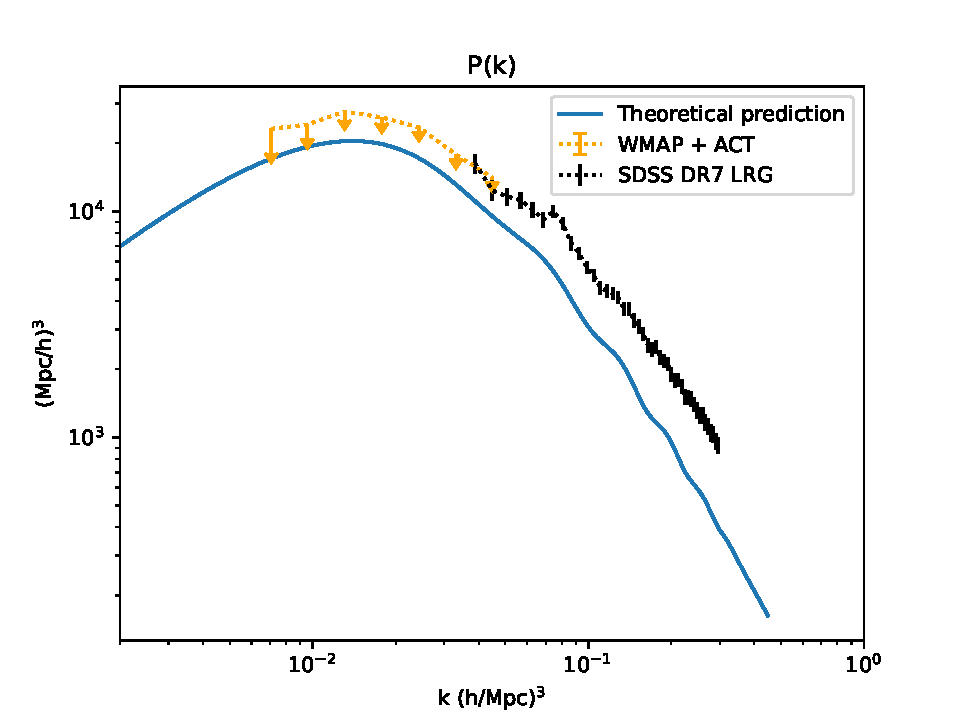
\includegraphics[scale=0.5]{Figures/milestone_4/Pk.pdf}
   \caption{ Comparison of the theory result for the linear matter power-spectrum with data from galaxy surveys (SDSS DR7 LRG) and the power-spectrum inferred from WMAP / ACT data.}
\label{fig:M4_Pk}
\end{figure}


\begin{figure}[h!]
   %\hspace{-0.48cm}   
   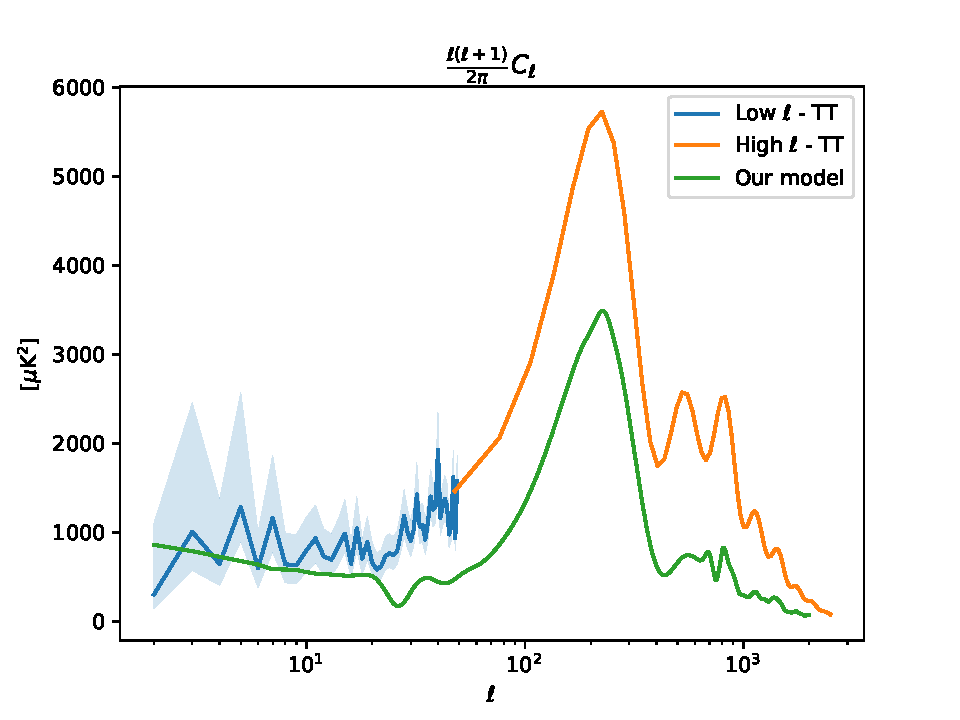
\includegraphics[scale=0.5]{Figures/milestone_4/C_ell.pdf}
   \caption{The CMB power spectrum as a function of $\ell$, computed using $\Lambda$CDM parameters along with the observed power spectrum from Planck along with error bars displaying the uncertainty. The computed power spectrum is normalized so that the first peak corresponds to the maxima from Planck at $\approx$ 6000 $\mu$K$^2$.}
\label{fig:M4_Cell}
\end{figure}
We see that the overall shape and behavior of the computed power spectrum follows the Planck data well even though the values are lower such as those in figure \ref{fig:M4_Pk}. The high amplitude for low $\ell$'s found in both the transfer function and the spectral integrand is visible as we see the amplitude of $\ell = 2$ being quite high. The biggest factor to why the peaks deviate from the observed peaks are likely because of our simplified model where we have ignored neutrinos and polarization. 

We also observe the final CMB power spectrum in \ref{fig:M4_Cell}. This model has the same shape as the low and high $\ell$ data from \cite{2}. The reason why the overall peaks of the power spectrum is lower, should be the same as in \ref{fig:M4_Pk}.





\section{Conclusions}
The successful development of a code capable of (to a certain degree) reproducing the CMB power spectrum is a significant achievement, and it signifies a notable advancement in our understanding of the physical processes and dynamics of the early universe. The CMB power spectrum serves as a direct probe of the primordial conditions and subsequent evolution of the universe. By achieving a faithful reproduction of this power spectrum, valuable insights into phenomena such as inflation and gravitational interactions at large scales are gained, deepening our understanding of the early universe.

In conclusion, the successful development of a code capable of reproducing the CMB power spectrum represents a significant scientific accomplishment. It deepens our knowledge of the early universe, demonstrates computational proficiency and it provides avenues for further scientific exploration through the depths of neutrinos and polarization.
\newpage
\begin{thebibliography}{}
%\bibliographystyle{apalike}
\bibitem[Betoule et al. (2014)]{1} Betoule, M et al. (2014) \textit{Improved cosmological constraints from a joint analysis of the SDSS-II and SNLS supernova samples}
\bibitem[Callin (2006)]{5} Callin, P. (2006) \textit{How to calculate the CMB spectrum}
\bibitem[Planck (2018)]{2} Planck Collaboration.( 2018) \textit{Planck 2018 results. VI. Cosmological parameters}
\bibitem[Winther (2023)]{3} Winther, H.A. 2023: \\
      \href{https://cmb.wintherscoming.no/milestone1.php}{https://cmb.wintherscoming.no/milestone1.php}
      \href{https://cmb.wintherscoming.no/milestone2.php}{https://cmb.wintherscoming.no/milestone2.php}
      \href{https://cmb.wintherscoming.no/milestone3.php}{https://cmb.wintherscoming.no/milestone3.php}
      \href{https://cmb.wintherscoming.no/milestone4.php}{https://cmb.wintherscoming.no/milestone4.php}
\bibitem[Tegmark\&Zaldarriaga (2003)]{4} Tegmark, M. Zaldarriaga, M. (2002) \textit{Separating the Early Universe from the Late Universe: cosmological parameter estimation beyond the black box}
\bibitem[Dodelson (2003)]{6} Dodelsen, S. \textit{Modern Cosmology} (2nd edition)

\end{thebibliography}


\end{document}
